
% -*- mode: latex; TeX-master: "Vorbis_I_spec"; -*-
%!TEX root = Vorbis_I_spec.tex
% $Id$
\section{Codec Setup and Packet Decode} \label{vorbis:spec:codec}

\subsection{Overview}

This document serves as the top-level reference document for the
bit-by-bit decode specification of Vorbis I.  This document assumes a
high-level understanding of the Vorbis decode process, which is
provided in \xref{vorbis:spec:intro}.  \xref{vorbis:spec:bitpacking} covers reading and writing bit fields from
and to bitstream packets.



\subsection{Header decode and decode setup}

A Vorbis bitstream begins with three header packets. The header
packets are, in order, the identification header, the comments header,
and the setup header. All are required for decode compliance.  An
end-of-packet condition during decoding the first or third header
packet renders the stream undecodable.  End-of-packet decoding the
comment header is a non-fatal error condition.

\subsubsection{Common header decode}

Each header packet begins with the same header fields.


\begin{Verbatim}[commandchars=\\\{\}]
  1) [packet\_type] : 8 bit value
  2) 0x76, 0x6f, 0x72, 0x62, 0x69, 0x73: the characters 'v','o','r','b','i','s' as six octets
\end{Verbatim}

Decode continues according to packet type; the identification header
is type 1, the comment header type 3 and the setup header type 5
(these types are all odd as a packet with a leading single bit of '0'
is an audio packet).  The packets must occur in the order of
identification, comment, setup.



\subsubsection{Identification header}

The identification header is a short header of only a few fields used
to declare the stream definitively as Vorbis, and provide a few externally
relevant pieces of information about the audio stream. The
identification header is coded as follows:

\begin{Verbatim}[commandchars=\\\{\}]
 1) [vorbis\_version] = read 32 bits as unsigned integer
 2) [audio\_channels] = read 8 bit integer as unsigned
 3) [audio\_sample\_rate] = read 32 bits as unsigned integer
 4) [bitrate\_maximum] = read 32 bits as signed integer
 5) [bitrate\_nominal] = read 32 bits as signed integer
 6) [bitrate\_minimum] = read 32 bits as signed integer
 7) [blocksize\_0] = 2 exponent (read 4 bits as unsigned integer)
 8) [blocksize\_1] = 2 exponent (read 4 bits as unsigned integer)
 9) [framing\_flag] = read one bit
\end{Verbatim}

\varname{[vorbis\_version]} is to read '0' in order to be compatible
with this document.  Both \varname{[audio\_channels]} and
\varname{[audio\_sample\_rate]} must read greater than zero.  Allowed final
blocksize values are 64, 128, 256, 512, 1024, 2048, 4096 and 8192 in
Vorbis I.  \varname{[blocksize\_0]} must be less than or equal to
\varname{[blocksize\_1]}.  The framing bit must be nonzero.  Failure to
meet any of these conditions renders a stream undecodable.

The bitrate fields above are used only as hints. The nominal bitrate
field especially may be considerably off in purely VBR streams.  The
fields are meaningful only when greater than zero.

\begin{itemize}
  \item All three fields set to the same value implies a fixed rate, or tightly bounded, nearly fixed-rate bitstream
  \item Only nominal set implies a VBR or ABR stream that averages the nominal bitrate
  \item Maximum and or minimum set implies a VBR bitstream that obeys the bitrate limits
  \item None set indicates the encoder does not care to speculate.
\end{itemize}




\subsubsection{Comment header}
Comment header decode and data specification is covered in
\xref{vorbis:spec:comment}.


\subsubsection{Setup header}

Vorbis codec setup is configurable to an extreme degree:

\begin{center}
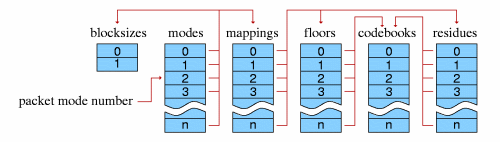
\includegraphics[width=\textwidth]{components}
\captionof{figure}{decoder pipeline configuration}
\end{center}


The setup header contains the bulk of the codec setup information
needed for decode.  The setup header contains, in order, the lists of
codebook configurations, time-domain transform configurations
(placeholders in Vorbis I), floor configurations, residue
configurations, channel mapping configurations and mode
configurations. It finishes with a framing bit of '1'.  Header decode
proceeds in the following order:

\paragraph{Codebooks}

\begin{enumerate}
\item \varname{[vorbis\_codebook\_count]} = read eight bits as unsigned integer and add one
\item Decode \varname{[vorbis\_codebook\_count]} codebooks in order as defined
in \xref{vorbis:spec:codebook}.  Save each configuration, in
order, in an array of
codebook configurations \varname{[vorbis\_codebook\_configurations]}.
\end{enumerate}



\paragraph{Time domain transforms}

These hooks are placeholders in Vorbis I.  Nevertheless, the
configuration placeholder values must be read to maintain bitstream
sync.

\begin{enumerate}
\item \varname{[vorbis\_time\_count]} = read 6 bits as unsigned integer and add one
\item read \varname{[vorbis\_time\_count]} 16 bit values; each value should be zero.  If any value is nonzero, this is an error condition and the stream is undecodable.
\end{enumerate}



\paragraph{Floors}

Vorbis uses two floor types; header decode is handed to the decode
abstraction of the appropriate type.

\begin{enumerate}
 \item \varname{[vorbis\_floor\_count]} = read 6 bits as unsigned integer and add one
 \item For each \varname{[i]} of \varname{[vorbis\_floor\_count]} floor numbers:
  \begin{enumerate}
   \item read the floor type: vector \varname{[vorbis\_floor\_types]} element \varname{[i]} =
read 16 bits as unsigned integer
   \item If the floor type is zero, decode the floor
configuration as defined in \xref{vorbis:spec:floor0}; save
this
configuration in slot \varname{[i]} of the floor configuration array \varname{[vorbis\_floor\_configurations]}.
   \item If the floor type is one,
decode the floor configuration as defined in \xref{vorbis:spec:floor1}; save this configuration in slot \varname{[i]} of the floor configuration array \varname{[vorbis\_floor\_configurations]}.
   \item If the the floor type is greater than one, this stream is undecodable; ERROR CONDITION
  \end{enumerate}

\end{enumerate}



\paragraph{Residues}

Vorbis uses three residue types; header decode of each type is identical.


\begin{enumerate}
\item \varname{[vorbis\_residue\_count]} = read 6 bits as unsigned integer and add one

\item For each of \varname{[vorbis\_residue\_count]} residue numbers:
 \begin{enumerate}
  \item read the residue type; vector \varname{[vorbis\_residue\_types]} element \varname{[i]} = read 16 bits as unsigned integer
  \item If the residue type is zero,
one or two, decode the residue configuration as defined in \xref{vorbis:spec:residue}; save this configuration in slot \varname{[i]} of the residue configuration array \varname{[vorbis\_residue\_configurations]}.
  \item If the the residue type is greater than two, this stream is undecodable; ERROR CONDITION
 \end{enumerate}

\end{enumerate}



\paragraph{Mappings}

Mappings are used to set up specific pipelines for encoding
multichannel audio with varying channel mapping applications. Vorbis I
uses a single mapping type (0), with implicit PCM channel mappings.

% FIXME/TODO: LaTeX cannot nest enumerate that deeply, so I have to use
% itemize at the innermost level. However, it would be much better to 
% rewrite this pseudocode using listings or algoritmicx or some other
% package geared towards this.
\begin{enumerate}
 \item \varname{[vorbis\_mapping\_count]} = read 6 bits as unsigned integer and add one
 \item For each \varname{[i]} of \varname{[vorbis\_mapping\_count]} mapping numbers:
  \begin{enumerate}
   \item read the mapping type: 16 bits as unsigned integer.  There's no reason to save the mapping type in Vorbis I.
   \item If the mapping type is nonzero, the stream is undecodable
   \item If the mapping type is zero:
    \begin{enumerate}
     \item read 1 bit as a boolean flag
      \begin{enumerate}
       \item if set, \varname{[vorbis\_mapping\_submaps]} = read 4 bits as unsigned integer and add one
       \item if unset, \varname{[vorbis\_mapping\_submaps]} = 1
      \end{enumerate}


     \item read 1 bit as a boolean flag
       \begin{enumerate}
         \item if set, square polar channel mapping is in use:
           \begin{itemize}
             \item \varname{[vorbis\_mapping\_coupling\_steps]} = read 8 bits as unsigned integer and add one
             \item for \varname{[j]} each of \varname{[vorbis\_mapping\_coupling\_steps]} steps:
               \begin{itemize}
                 \item vector \varname{[vorbis\_mapping\_magnitude]} element \varname{[j]}= read \link{vorbis:spec:ilog}{ilog}(\varname{[audio\_channels]} - 1) bits as unsigned integer
                 \item vector \varname{[vorbis\_mapping\_angle]} element \varname{[j]}= read \link{vorbis:spec:ilog}{ilog}(\varname{[audio\_channels]} - 1) bits as unsigned integer
                 \item the numbers read in the above two steps are channel numbers representing the channel to treat as magnitude and the channel to treat as angle, respectively.  If for any coupling step the angle channel number equals the magnitude channel number, the magnitude channel number is greater than \varname{[audio\_channels]}-1, or the angle channel is greater than \varname{[audio\_channels]}-1, the stream is undecodable.
               \end{itemize}


           \end{itemize}


         \item if unset, \varname{[vorbis\_mapping\_coupling\_steps]} = 0
       \end{enumerate}


     \item read 2 bits (reserved field); if the value is nonzero, the stream is undecodable
     \item if \varname{[vorbis\_mapping\_submaps]} is greater than one, we read channel multiplex settings. For each \varname{[j]} of \varname{[audio\_channels]} channels:
      \begin{enumerate}
       \item vector \varname{[vorbis\_mapping\_mux]} element \varname{[j]} = read 4 bits as unsigned integer
       \item if the value is greater than the highest numbered submap (\varname{[vorbis\_mapping\_submaps]} - 1), this in an error condition rendering the stream undecodable
      \end{enumerate}

     \item for each submap \varname{[j]} of \varname{[vorbis\_mapping\_submaps]} submaps, read the floor and residue numbers for use in decoding that submap:
      \begin{enumerate}
       \item read and discard 8 bits (the unused time configuration placeholder)
       \item read 8 bits as unsigned integer for the floor number; save in vector \varname{[vorbis\_mapping\_submap\_floor]} element \varname{[j]}
       \item verify the floor number is not greater than the highest number floor configured for the bitstream. If it is, the bitstream is undecodable
       \item read 8 bits as unsigned integer for the residue number; save in vector \varname{[vorbis\_mapping\_submap\_residue]} element \varname{[j]}
       \item verify the residue number is not greater than the highest number residue configured for the bitstream.  If it is, the bitstream is undecodable
      \end{enumerate}

     \item save this mapping configuration in slot \varname{[i]} of the mapping configuration array \varname{[vorbis\_mapping\_configurations]}.
    \end{enumerate}

  \end{enumerate}

\end{enumerate}



\paragraph{Modes}

\begin{enumerate}
 \item \varname{[vorbis\_mode\_count]} = read 6 bits as unsigned integer and add one
 \item For each of \varname{[vorbis\_mode\_count]} mode numbers:
  \begin{enumerate}
  \item \varname{[vorbis\_mode\_blockflag]} = read 1 bit
  \item \varname{[vorbis\_mode\_windowtype]} = read 16 bits as unsigned integer
  \item \varname{[vorbis\_mode\_transformtype]} = read 16 bits as unsigned integer
  \item \varname{[vorbis\_mode\_mapping]} = read 8 bits as unsigned integer
  \item verify ranges; zero is the only legal value in Vorbis I for
\varname{[vorbis\_mode\_windowtype]}
and \varname{[vorbis\_mode\_transformtype]}.  \varname{[vorbis\_mode\_mapping]} must not be greater than the highest number mapping in use.  Any illegal values render the stream undecodable.
  \item save this mode configuration in slot \varname{[i]} of the mode configuration array
\varname{[vorbis\_mode\_configurations]}.
 \end{enumerate}

\item read 1 bit as a framing flag.  If unset, a framing error occurred and the stream is not
decodable.
\end{enumerate}

After reading mode descriptions, setup header decode is complete.








\subsection{Audio packet decode and synthesis}

Following the three header packets, all packets in a Vorbis I stream
are audio.  The first step of audio packet decode is to read and
verify the packet type. \emph{A non-audio packet when audio is expected
indicates stream corruption or a non-compliant stream. The decoder
must ignore the packet and not attempt decoding it to audio}.


\subsubsection{packet type, mode and window decode}

\begin{enumerate}
 \item read 1 bit \varname{[packet\_type]}; check that packet type is 0 (audio)
 \item read \link{vorbis:spec:ilog}{ilog}([vorbis\_mode\_count]-1) bits
\varname{[mode\_number]}
 \item decode blocksize \varname{[n]} is equal to \varname{[blocksize\_0]} if
\varname{[vorbis\_mode\_blockflag]} is 0, else \varname{[n]} is equal to \varname{[blocksize\_1]}.
 \item perform window selection and setup; this window is used later by the inverse MDCT:
  \begin{enumerate}
   \item if this is a long window (the \varname{[vorbis\_mode\_blockflag]} flag of this mode is
set):
    \begin{enumerate}
     \item read 1 bit for \varname{[previous\_window\_flag]}
     \item read 1 bit for \varname{[next\_window\_flag]}
     \item if \varname{[previous\_window\_flag]} is not set, the left half
         of the window will be a hybrid window for lapping with a
         short block.  See \xref{vorbis:spec:window} for an illustration of overlapping
dissimilar
         windows. Else, the left half window will have normal long
         shape.
     \item if \varname{[next\_window\_flag]} is not set, the right half of
         the window will be a hybrid window for lapping with a short
         block.  See \xref{vorbis:spec:window} for an
illustration of overlapping dissimilar
         windows. Else, the left right window will have normal long
         shape.
    \end{enumerate}

   \item  if this is a short window, the window is always the same
       short-window shape.
  \end{enumerate}

\end{enumerate}

Vorbis windows all use the slope function $y=\sin(\frac{\pi}{2} * \sin^2((x+0.5)/n * \pi))$,
where $n$ is window size and $x$ ranges $0 \ldots n-1$, but dissimilar
lapping requirements can affect overall shape.  Window generation
proceeds as follows:

\begin{enumerate}
 \item  \varname{[window\_center]} = \varname{[n]} / 2
 \item  if (\varname{[vorbis\_mode\_blockflag]} is set and \varname{[previous\_window\_flag]} is
not set) then
  \begin{enumerate}
   \item \varname{[left\_window\_start]} = \varname{[n]}/4 -
\varname{[blocksize\_0]}/4
   \item \varname{[left\_window\_end]} = \varname{[n]}/4 + \varname{[blocksize\_0]}/4
   \item \varname{[left\_n]} = \varname{[blocksize\_0]}/2
  \end{enumerate}
 else
  \begin{enumerate}
   \item \varname{[left\_window\_start]} = 0
   \item \varname{[left\_window\_end]} = \varname{[window\_center]}
   \item \varname{[left\_n]} = \varname{[n]}/2
  \end{enumerate}

 \item  if (\varname{[vorbis\_mode\_blockflag]} is set and \varname{[next\_window\_flag]} is not
set) then
  \begin{enumerate}
   \item \varname{[right\_window\_start]} = \varname{[n]*3}/4 -
\varname{[blocksize\_0]}/4
   \item \varname{[right\_window\_end]} = \varname{[n]*3}/4 +
\varname{[blocksize\_0]}/4
   \item \varname{[right\_n]} = \varname{[blocksize\_0]}/2
  \end{enumerate}
 else
  \begin{enumerate}
   \item \varname{[right\_window\_start]} = \varname{[window\_center]}
   \item \varname{[right\_window\_end]} = \varname{[n]}
   \item \varname{[right\_n]} = \varname{[n]}/2
  \end{enumerate}

 \item  window from range 0 ... \varname{[left\_window\_start]}-1 inclusive is zero
 \item  for \varname{[i]} in range \varname{[left\_window\_start]} ...
\varname{[left\_window\_end]}-1, window(\varname{[i]}) = $\sin(\frac{\pi}{2} * \sin^2($ (\varname{[i]}-\varname{[left\_window\_start]}+0.5) / \varname{[left\_n]} $* \frac{\pi}{2})$ )
 \item  window from range \varname{[left\_window\_end]} ... \varname{[right\_window\_start]}-1
inclusive is one\item  for \varname{[i]} in range \varname{[right\_window\_start]} ... \varname{[right\_window\_end]}-1, window(\varname{[i]}) = $\sin(\frac{\pi}{2} * \sin^2($ (\varname{[i]}-\varname{[right\_window\_start]}+0.5) / \varname{[right\_n]} $ * \frac{\pi}{2} + \frac{\pi}{2})$ )
\item  window from range \varname{[right\_window\_start]} ... \varname{[n]}-1 is
zero
\end{enumerate}

An end-of-packet condition up to this point should be considered an
error that discards this packet from the stream.  An end of packet
condition past this point is to be considered a possible nominal
occurrence.



\subsubsection{floor curve decode}

From this point on, we assume out decode context is using mode number
\varname{[mode\_number]} from configuration array
\varname{[vorbis\_mode\_configurations]} and the map number
\varname{[vorbis\_mode\_mapping]} (specified by the current mode) taken
from the mapping configuration array
\varname{[vorbis\_mapping\_configurations]}.

Floor curves are decoded one-by-one in channel order.

For each floor \varname{[i]} of \varname{[audio\_channels]}
 \begin{enumerate}
  \item \varname{[submap\_number]} = element \varname{[i]} of vector [vorbis\_mapping\_mux]
  \item \varname{[floor\_number]} = element \varname{[submap\_number]} of vector
[vorbis\_submap\_floor]
  \item if the floor type of this
floor (vector \varname{[vorbis\_floor\_types]} element
\varname{[floor\_number]}) is zero then decode the floor for
channel \varname{[i]} according to the
\xref{vorbis:spec:floor0-decode}
  \item if the type of this floor
is one then decode the floor for channel \varname{[i]} according
to the \xref{vorbis:spec:floor1-decode}
  \item save the needed decoded floor information for channel for later synthesis
  \item if the decoded floor returned 'unused', set vector \varname{[no\_residue]} element
\varname{[i]} to true, else set vector \varname{[no\_residue]} element \varname{[i]} to
false
 \end{enumerate}


An end-of-packet condition during floor decode shall result in packet
decode zeroing all channel output vectors and skipping to the
add/overlap output stage.



\subsubsection{nonzero vector propagate}

A possible result of floor decode is that a specific vector is marked
'unused' which indicates that that final output vector is all-zero
values (and the floor is zero).  The residue for that vector is not
coded in the stream, save for one complication.  If some vectors are
used and some are not, channel coupling could result in mixing a
zeroed and nonzeroed vector to produce two nonzeroed vectors.

for each \varname{[i]} from 0 ... \varname{[vorbis\_mapping\_coupling\_steps]}-1

\begin{enumerate}
 \item if either \varname{[no\_residue]} entry for channel
(\varname{[vorbis\_mapping\_magnitude]} element \varname{[i]})
or channel
(\varname{[vorbis\_mapping\_angle]} element \varname{[i]})
are set to false, then both must be set to false.  Note that an 'unused'
floor has no decoded floor information; it is important that this is
remembered at floor curve synthesis time.
\end{enumerate}




\subsubsection{residue decode}

Unlike floors, which are decoded in channel order, the residue vectors
are decoded in submap order.

for each submap \varname{[i]} in order from 0 ... \varname{[vorbis\_mapping\_submaps]}-1

\begin{enumerate}
 \item \varname{[ch]} = 0
 \item for each channel \varname{[j]} in order from 0 ... \varname{[audio\_channels]} - 1
  \begin{enumerate}
   \item if channel \varname{[j]} in submap \varname{[i]} (vector \varname{[vorbis\_mapping\_mux]} element \varname{[j]} is equal to \varname{[i]})
    \begin{enumerate}
     \item if vector \varname{[no\_residue]} element \varname{[j]} is true
      \begin{enumerate}
       \item vector \varname{[do\_not\_decode\_flag]} element \varname{[ch]} is set
      \end{enumerate}
     else
      \begin{enumerate}
       \item vector \varname{[do\_not\_decode\_flag]} element \varname{[ch]} is unset
      \end{enumerate}

     \item increment \varname{[ch]}
    \end{enumerate}

  \end{enumerate}
 \item \varname{[residue\_number]} = vector \varname{[vorbis\_mapping\_submap\_residue]} element \varname{[i]}
 \item \varname{[residue\_type]} = vector \varname{[vorbis\_residue\_types]} element \varname{[residue\_number]}
 \item decode \varname{[ch]} vectors using residue \varname{[residue\_number]}, according to type \varname{[residue\_type]}, also passing vector \varname{[do\_not\_decode\_flag]} to indicate which vectors in the bundle should not be decoded. Correct per-vector decode length is \varname{[n]}/2.
 \item \varname{[ch]} = 0
 \item for each channel \varname{[j]} in order from 0 ... \varname{[audio\_channels]}
  \begin{enumerate}
   \item if channel \varname{[j]} is in submap \varname{[i]} (vector \varname{[vorbis\_mapping\_mux]} element \varname{[j]} is equal to \varname{[i]})
    \begin{enumerate}
     \item residue vector for channel \varname{[j]} is set to decoded residue vector \varname{[ch]}
     \item increment \varname{[ch]}
    \end{enumerate}

  \end{enumerate}

\end{enumerate}



\subsubsection{inverse coupling}

for each \varname{[i]} from \varname{[vorbis\_mapping\_coupling\_steps]}-1 descending to 0

\begin{enumerate}
 \item \varname{[magnitude\_vector]} = the residue vector for channel
(vector \varname{[vorbis\_mapping\_magnitude]} element \varname{[i]})
 \item \varname{[angle\_vector]} = the residue vector for channel (vector
\varname{[vorbis\_mapping\_angle]} element \varname{[i]})
 \item for each scalar value \varname{[M]} in vector \varname{[magnitude\_vector]} and the corresponding scalar value \varname{[A]} in vector \varname{[angle\_vector]}:
  \begin{enumerate}
   \item if (\varname{[M]} is greater than zero)
    \begin{enumerate}
     \item if (\varname{[A]} is greater than zero)
      \begin{enumerate}
       \item \varname{[new\_M]} = \varname{[M]}
       \item \varname{[new\_A]} = \varname{[M]}-\varname{[A]}
      \end{enumerate}
     else
      \begin{enumerate}
       \item \varname{[new\_A]} = \varname{[M]}
       \item \varname{[new\_M]} = \varname{[M]}+\varname{[A]}
      \end{enumerate}

    \end{enumerate}
   else
    \begin{enumerate}
     \item if (\varname{[A]} is greater than zero)
      \begin{enumerate}
       \item \varname{[new\_M]} = \varname{[M]}
       \item \varname{[new\_A]} = \varname{[M]}+\varname{[A]}
      \end{enumerate}
     else
      \begin{enumerate}
       \item \varname{[new\_A]} = \varname{[M]}
       \item \varname{[new\_M]} = \varname{[M]}-\varname{[A]}
      \end{enumerate}

    \end{enumerate}

   \item set scalar value \varname{[M]} in vector \varname{[magnitude\_vector]} to \varname{[new\_M]}
   \item set scalar value \varname{[A]} in vector \varname{[angle\_vector]} to \varname{[new\_A]}
  \end{enumerate}

\end{enumerate}




\subsubsection{dot product}

For each channel, synthesize the floor curve from the decoded floor
information, according to packet type. Note that the vector synthesis
length for floor computation is \varname{[n]}/2.

For each channel, multiply each element of the floor curve by each
element of that channel's residue vector.  The result is the dot
product of the floor and residue vectors for each channel; the produced
vectors are the length \varname{[n]}/2 audio spectrum for each
channel.

% TODO/FIXME: The following two paragraphs have identical twins
%   in section 1 (under "compute floor/residue dot product")
One point is worth mentioning about this dot product; a common mistake
in a fixed point implementation might be to assume that a 32 bit
fixed-point representation for floor and residue and direct
multiplication of the vectors is sufficient for acceptable spectral
depth in all cases because it happens to mostly work with the current
Xiph.Org reference encoder.

However, floor vector values can span \~140dB (\~24 bits unsigned), and
the audio spectrum vector should represent a minimum of 120dB (\~21
bits with sign), even when output is to a 16 bit PCM device.  For the
residue vector to represent full scale if the floor is nailed to
$-140$dB, it must be able to span 0 to $+140$dB.  For the residue vector
to reach full scale if the floor is nailed at 0dB, it must be able to
represent $-140$dB to $+0$dB.  Thus, in order to handle full range
dynamics, a residue vector may span $-140$dB to $+140$dB entirely within
spec.  A 280dB range is approximately 48 bits with sign; thus the
residue vector must be able to represent a 48 bit range and the dot
product must be able to handle an effective 48 bit times 24 bit
multiplication.  This range may be achieved using large (64 bit or
larger) integers, or implementing a movable binary point
representation.



\subsubsection{inverse MDCT}

Convert the audio spectrum vector of each channel back into time
domain PCM audio via an inverse Modified Discrete Cosine Transform
(MDCT).  A detailed description of the MDCT is available in \cite{Sporer/Brandenburg/Edler}.  The window
function used for the MDCT is the function described earlier.



\subsubsection{overlap\_add}

Windowed MDCT output is overlapped and added with the right hand data
of the previous window such that the 3/4 point of the previous window
is aligned with the 1/4 point of the current window (as illustrated in
\xref{vorbis:spec:window}).  The overlapped portion
produced from overlapping the previous and current frame data is
finished data to be returned by the decoder.  This data spans from the
center of the previous window to the center of the current window.  In
the case of same-sized windows, the amount of data to return is
one-half block consisting of and only of the overlapped portions. When
overlapping a short and long window, much of the returned range does not
actually overlap.  This does not damage transform orthogonality.  Pay
attention however to returning the correct data range; the amount of
data to be returned is:

\begin{programlisting}
window_blocksize(previous_window)/4+window_blocksize(current_window)/4
\end{programlisting}

from the center (element windowsize/2) of the previous window to the
center (element windowsize/2-1, inclusive) of the current window.

Data is not returned from the first frame; it must be used to 'prime'
the decode engine.  The encoder accounts for this priming when
calculating PCM offsets; after the first frame, the proper PCM output
offset is '0' (as no data has been returned yet).



\subsubsection{output channel order}

Vorbis I specifies only a channel mapping type 0.  In mapping type 0,
channel mapping is implicitly defined as follows for standard audio
applications. As of revision 16781 (20100113), the specification adds
defined channel locations for 6.1 and 7.1 surround.  Ordering/location
for greater-than-eight channels remains 'left to the implementation'.

These channel orderings refer to order within the encoded stream.  It
is naturally possible for a decoder to produce output with channels in
any order. Any such decoder should explicitly document channel
reordering behavior.

\begin{description} %[style=nextline]
 \item[one channel]
	the stream is monophonic

\item[two channels]
	the stream is stereo.  channel order: left, right

\item[three channels]
	the stream is a 1d-surround encoding.  channel order: left,
center, right

\item[four channels]
	the stream is quadraphonic surround.  channel order: front left,
front right, rear left, rear right

\item[five channels]
	the stream is five-channel surround.  channel order: front left,
center, front right, rear left, rear right

\item[six channels]
	the stream is 5.1 surround.  channel order: front left, center, 
front right, rear left, rear right, LFE

\item[seven channels]
        the stream is 6.1 surround.  channel order: front left, center, 
front right, side left, side right, rear center, LFE

\item[eight channels]
        the stream is 7.1 surround.  channel order: front left, center, 
front right, side left, side right, rear left, rear right, 
LFE

\item[greater than eight channels]
	channel use and order is defined by the application

\end{description}

Applications using Vorbis for dedicated purposes may define channel
mapping as seen fit.  Future channel mappings (such as three and four
channel \href{http://www.ambisonic.net/}{Ambisonics}) will
make use of channel mappings other than mapping 0.


